\DiaryEntry{Catalan Numbers - Intro}{2022-06-15}{Combinatorics}

In combinatorial mathematics, the Catalan numbers are a sequence of natural numbers that occur in various counting problems, often involving recursively defined objects.

\subsection{Definition}

There is a recurrence relation for the Catalan numbers,

\be\label{2022-06-15:eq1}
C_{n+1} = \sum_{i=0}^n C_i C_{n-i}, \,\, n \geq 0, \quad C_0=1
\ee

but the Catalan numbers can also be expressed directly as

\bee
C_n = \frac{1}{n+1} {2n \choose n} = {2n \choose n} - {2n \choose n+1}
\eee

The first Catalan numbers are

\bee
    1, 1, 2, 5, 14, 42, 132, 429, 1430, 4862, 16796, 58786, \ldots
\eee

and they are sequence \href{https://oeis.org/A000108}{A000108} in the OEIS.

\subsection{Application, Proofs}

There are literally hundreds of things which the Catalan numbers count. See Stanley, Catalan Numbers \todo{make proper bibtex ref}.

\paragraph{Counting Polygon Triangulations.} Let $\Pc_n$ denote a convex polygon with $n$ vertices. A triangulation of $\Pc_n$ is a set of $n-3$ diagonals which do not cross. A triangulation partitions the polygon $\Pc_{n+2}$ into $n$ triangles and we define the $n$th Catalan number as the number of triangulations of $\Pc_{n+2}$.

The triangulations for $\Pc_3, \Pc_4$ and $\Pc_5$ are shown in the following Figure.

\begin{figure}[H]v
\centering
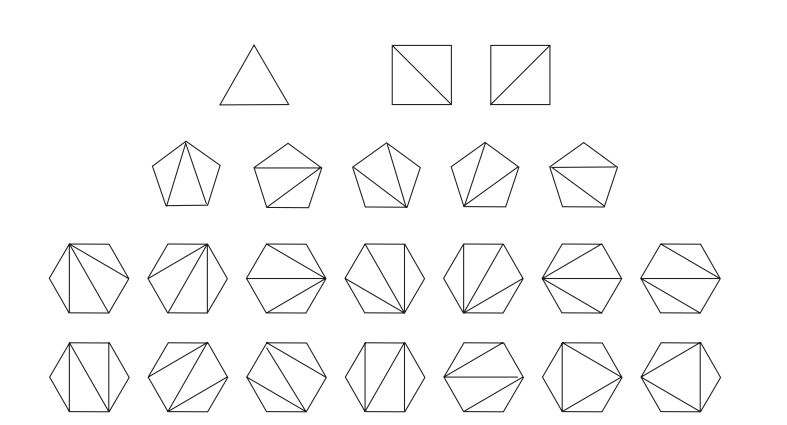
\includegraphics[scale=0.5]{images/2022-06-15-catalan_01.png}
\end{figure}

This counting argument allows to prove the recurrence relation \eqref{2022-06-15:eq1} as follows. Consider an $n+3$-polygon $\Pc_{n+3}$ (having $C_{n+1}$ triangulations). We can split this polygon into two polygons $\Qc_1$ and $\Qc_2$, having $a_1+2$ and $a_2+2$ vertices, respectively. Therefore, $\Qc_1$ has $C_{a_1}$ triangulations and  $\Qc_2$ has $C_{a_2}$ triangulations.

We can reverse the process and construct a triangulation of $\Pc_{n+3}$ by combining the triangulations of $\Qc_1$ and $\Qc_2$. The triangulations are ``independent''; i.e. we can fix one triangulation of $\Qc_1$ and choose on of the $C_{a_2}$ triangulations. of $\Qc_2$. We therefore have for the number of triangulations of $\Pc_{n+3}$ as

\bee
C_{n+1} = \sum_{k=0}^n C_k C_{n-k} \qed
\eee




%%% Local Variables:
%%% mode: latex
%%% TeX-master: "journal"
%%% End:
